\section*{Utilisation en ligne de commande}
L'application propose quelques options en ligne de commande.

\paragraph{--snake} [chemin] permet de charger un snake autre que celui par défaut au démarrage du programme. A noté qu'il est possible de charger d'autre snake une fois le programme démarré (voir plus loin).

\paragraph{--threadNb} [nombre max de thread] permet d'indiquer le nombre maximal de thread que vous souhaitez que l'application utilise pour chercher les solutions. Par défaut le nombre de thread utilisé est égale au nombre de point de départ pour le snake sélectionné.

\paragraph{--help} pour avoir l'aide.

\section*{Menu graphique}
Une fois lancé, l'application propose un menu qui vous permettra de faire les choses suivantes :

\begin{figure}[h]
 \centering
 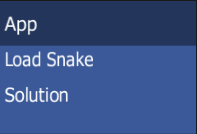
\includegraphics[scale=0.7,keepaspectratio=true]{img/menu1.png}
 \caption{Menu de l'application}
\end{figure}